
\documentclass{article}% APA Reference Style 

\usepackage{graphicx}%
\usepackage{multirow}%
\usepackage{amsmath,amssymb,amsfonts}%
\usepackage{amsthm}%
\usepackage{authblk}
\usepackage{mathrsfs}%
\usepackage[title]{appendix}%
\usepackage{xcolor}%
\usepackage{textcomp}%
\usepackage{manyfoot}%
\usepackage{booktabs}%
\usepackage[round]{natbib}
\usepackage{algorithm}%
\usepackage{algorithmicx}%
\usepackage{algpseudocode}%
\usepackage{listings}%
\usepackage{lineno}
\usepackage{orcidlink}
%\usepackage{url}
%%%%

%\theoremstyle{thmstyleone}%
%\newtheorem{theorem}{Theorem}%  
%\newtheorem{proposition}[theorem]{Proposition}% 


%\theoremstyle{thmstyletwo}%
%\newtheorem{example}{Example}%
%\newtheorem{remark}{Remark}%

%\theoremstyle{thmstylethree}%
%\newtheorem{definition}{Definition}%

%\raggedbottom
%%\unnumbered% uncomment this for unnumbered level heads

\begin{document}

\title{A Comprehensive Analysis of the Italian School System Using Harmonized Open Data via the SchoolDataIT R Package}

%%=============================================================%%
%% GivenName	-> \fnm{Joergen W.}
%% Particle	-> \spfx{van der} -> surname prefix
%% FamilyName	-> \sur{Ploeg}
%% Suffix	-> \sfx{IV}
%% \author*[1,2]{\fnm{Joergen W.} \spfx{van der} \sur{Ploeg} 
%%  \sfx{IV}}\email{iauthor@gmail.com}
%%=============================================================%%

\author[1]{Leonardo Cefalo }

\author[1]{Alessio Pollice}
%\equalcont{These authors contributed equally to this work.}

\author[2]{Paolo Maranzano}
%\equalcont{These authors contributed equally to this work.}

\affil[1]{Department of Economics and Finance, Università degli Studi di Bari Aldo Moro, Bari, Italy}

\affil[2]{Dipartimento di Scienze Statistiche, Università degli studi di Milano Bicocca, Milan, Italy}


%%==================================%%
%% Sample for unstructured abstract %%
%%==================================%%

\maketitle
\begin{abstract}
We propose an overview on the current status of the Italian educational system, with particular regard to school infrastructure, using the dedicated \texttt{R} library \texttt{SchoolDataIT}, which aims at gathering the relevant open data through web scraping and harmonizing them into an organic database. In addition to infrastructural information, the software retrieves the results of the Invalsi census survey, which is typically considered a thorough indicator of education quality nationwide. The package is composed of four main groups of functions. The first group retrieves the inputs from the source web pages; the second one is employed for basic data editing; the third one aggregates the data at a given territorial level, either municipalities (LAU) or provinces (NUTS-3); lastly, mapping functions are included to render the final datasets through static or interactive maps. We show the potential application of the software by providing a practical example that highlights the importance of spatial statistics to model data about the educational system at the territorial level. Indeed, territorial disparities can be found across several dimensions of both infrastructure endowment and education quality, representing a significant challenge to territorial sustainability.
\end{abstract}

\noindent \textbf{keywords:} Italian School System, School Infrastructure, Web Scraping, \texttt{SchoolDataIT} library, \texttt{R} programming language



\section{Introduction}
The proper management of the public education system requires a full understanding of the territorial endowment in school infrastructure and the quality of education. Infrastructure endowment, in particular, is a direct area of policy intervention at various administrative levels. The depth of the link between the endowment in the material infrastructure and the quality of education is a matter of common knowledge and encompasses numerous dimensions of the education system, as highlighted in \cite{WB}. The evidence gathered therein across different countries sheds light on the relevance of several material factors on student achievements and education equity.

The first infrastructural dimension to be taken into account is the accessibility of schools and learning spaces, also in terms of school size, since less crowded schools both enforce the bond between students and the learning environment and allow for a more dense distribution of schools over the territory, which reduces the average travel distance from households. A closely related issue is classroom size, which is typically shown in the literature to negatively affect education quality \citep{WB}.

Another dimension drawing attention from the literature is safety in school buildings, which can be assessed both with respect to outdoor hazards like pollution or natural events such as earthquakes, and in terms of indoor environmental quality, which can be summarized by factors such as illumination, indoor air quality (the main threat being the concentration of $\mathrm{CO_{2}}$, which also can undermine student attention), air temperature and acoustic quality, which however may strongly depend on outside acoustic disturbances. Another element to be taken into account is the impact of health hazards on school attendance, which is also relevant in developed countries, mainly on the side of respiratory diseases. Lastly, it is worth remarking on the importance of adequate physical extra-classroom spaces, such as IT laboratories, and recreational spaces like gymnasia or canteens, which intuitively allow for full-time schooling, which in turn is interpreted as a gain in school years attended by pupils.

The Italian school system offers a self-evident case for the significance of territorial disparities in education quality, both in terms of infrastructure endowment and student outcomes. Regarding the first case,  \cite{Garlaschi} and \cite{BDI} provide a detailed analysis of the distribution of school infrastructure on the national territory; Importantly, the northern regions show an advantage in terms of recreational spaces, learning spaces, safety certifications and school accessibility. In addition, \cite{BDI} show that such infrastructural characteristics have an impact on the results of the students. Regarding student outcomes, it is worth noting that the North-South divide is widely acknowledged to shape dramatically the distribution of student performances, e.g., as shown in \cite{Agasisti}. In particular, this disparity increases along the schooling process, implicitly suggesting that educational gaps tend to accumulate over time \citep{Invalsi2020}. In addition to the North-South gap,  evidence for spatial patterns in student outcome results can also be detected within the Northern and Southern macroregions and territorial clusters in both cases \citep[][respectively]{bag:do:north, do:bag:mar:south}. Overall evidence suggests therefore the need for policy actions directed at improving the material conditions of schools in the most vulnerable areas.

Thus, allocating adequate resources is a sensitive challenge for policymakers, also considering the heterogeneous funding system of school buildings and the uneven spending capacities between regions \citep[as in the case of Northern special statute regions, see][]{BDI}.

Motivated by the previous considerations, we believe that a structured set of multidimensional data about the Italian school system gathered from several institutional sources, along with georeferenced information, would be a valuable tool to detect the main areas of vulnerability and to plan appropriate development policies across the country. To this aim, we have developed \texttt{SchoolDataIT}, a software written in the \texttt{R} programming language \citep{R} which retrieves and harmonizes some relevant institutional databases at the territorial level of either municipalities (LAU hereinafter) and provinces \citep[NUTS-3 henceforth, ][]{NUTS2024}. 
The \texttt{SchoolDataIT} package is intended as a contribution to a broader repository, namely the AMELIA platform (\url{https://grins.it/progetto/piattaforma-amelia}), an open-data platform designed to produce and harmonize high-quality statistical data and analyses, managed by the \textit{Growing Resilient, Inclusive, and Sustainable} (GRINS) Foundation, a multidisciplinary initiative funded by the NextGenerationEU (NGEU) Recovery Plan \citep{CrescenziEtAl2021, DeLaPorteJensen2021}. 
Data providers are the Italian Ministry of Education (formerly MIUR, Ministry of Education, University and Research) \citep{MIUR}, the Institute for the Evaluation of the Education System (hereinafter Invalsi) \citep{Invalsi_IS}, the Italian National Institute of Statistics \citep[ISTAT,][]{InnerAreas, Situas, Shapefiles}, and the in-house company Infratel SPA on behalf of the Italian Ministry of Enterprises and Made in Italy \citep[MIMIT,][]{BB}, which is responsible of implementing and managing the ultra-broad band strategic plan. Since all of the data we take as input are open and publicly accessible, we retrieve them via web scraping, allowing for real-time updated inputs while requiring no storage space in the local machine of the user.

%%%%%% Versione 0.2.2 era quella disponibile alla data di submission
%%%%%% Ad oggi su CRAN è presente 0.2.4 (0.2.5 su github)
The \texttt{SchoolDataIT} software is currently available under version 0.2.4, released on March 28th 2025 on the Comprehensive R Archive Network \href{https://cran.r-project.org/web/packages/SchoolDataIT/index.html}{(CRAN)}. To ensure constant package maintenance, experimental version 0.2.5 is hosted on \href{https://github.com/lcef97/SchoolDataIT}{GitHub}.

The remainder of this paper is structured as follows. In Section \ref{sec:Overview}, we offer a concise yet comprehensive overview of the infrastructural state of Italian schools in light of the scientific literature on the national case and on official documents from the Ministry. In Section \ref{sec:Workflow}, we describe in detail the structure of the library and the most relevant functions made available for the users. In Section \ref{sec:Data}, we describe the datasets that can be accessed through the package, while including some relevant examples and potentiality. Finally, in Section \ref{sec:Example}, an empirical exercise involving the implementation of Bayesian spatial regression models is presented to investigate the student outcomes across the Italian territory.

\section{School infrastructure in Italy} \label{sec:Overview}


In this section, we briefly assess the current state of public school infrastructures in Italy using data provided by the Ministry of Education and processed through the \texttt{SchoolDataIT} package. Notice that, for the sake of brevity, in the main manuscript we only comment on the main findings that can be inferred from the original data. However, detailed information is resumed in the tables reported in Appendix \ref{Appendix1}.

The first dimension we take into consideration is school size. According to \cite{BDI}, in the Italian context, Northern regions leverage on a marked advantage in terms of school surface per student, particularly for kindergarten and primary schools. This result is particularly interesting if we consider how Northern schools are more crowded than Southern ones and have a lower teachers/students ratio (in this regard, see also Section \ref{par:nstud}). On the one side, the number of municipalities hosting a primary or a middle school is relatively high. Indeed, according to the National School Registry \ref{par:registry}, for school year 2021/2022, roughly 6748 ($85.38\%$ of the national total) and 5258 municipalities ($66.52\%$ of the total) host at least one primary and one middle school respectively. Conversely, high schools are located in only $1473$ municipalities ($18.64\%$ of the total), thus having a more sparse distribution, especially in the peripheral inland. However, \cite{BDI} showed that only in 139 municipalities ($1.76\%$ of the total) the travel time to the nearest school exceeds the threshold of 30 minutes. This finding is consistent with the smaller size of schools in such territories, which allows for a relatively widespread distribution of school buildings. If we move our focus to access to full-time schooling in primary schools, the North-South divide becomes an obvious cross-regional phenomenon. As reported in Table \ref{tab:fulltime} in Appendix \ref{Appendix1}, among the 18 regions for which data are available, 8 out of the 9 regions with the lowest values are located in the South (except Umbria), while 8 out of the 9 regions with the highest values are in the Center-North (except Basilicata).

Another fundamental factor in school accessibility is the availability of public transport. As declared by \cite{MIUR}, see also Section \ref{par:buildings}, interurban and railway transport is considered available if the nearest hub is located within 500 meters from the school, while urban transport is considered available if the hub lies within a range of 250 meters. As documented in \cite{Garlaschi}, Northern regions generally outperform Southern ones in terms of urban and interurban public transport availability, though significant differences are observed within macro-regions. For instance, within the Southern regions, Abruzzo owns the percentage of schools served by public transport systematically exceeding the national average, while Campania and Calabria appear to display the most vulnerable profile. The availability of urban, interurban, and disabled-people-specific transport at the regional level is shown in Table \ref{tab:transport} in Appendix \ref{Appendix1}.

Regarding school building safety, one can consider at least two kinds of hazards. The first is pollution exposure. In particular, three main risk factors are explicitly monitored by the Ministry of Education, namely the proximity to either hazardous industries, pollutant waters, or sources of air pollution. These specific issues occur in a relatively small number of localized cases and would deserve a more dedicated analysis due to their severity. A general finding to be considered is that air pollution poses an important threat in terms both of health and physical well-being and education quality indeed, as recent evidence \citep{AQInvalsi} shows that not only does the presence of particulate matter (PM$_{2.5}$)  impact student outcomes, but the significance of this impact increases as the socio-economic status of students decreases.

Another serious hazard affecting the whole Italian territory is the unpredictable occurrence of an earthquake. Based on 2023 data, almost half of the school buildings are located in high or medium-high seismic risk areas\footnote{In Italy, the seismic risk of a given area is classified based on the relative peak ground acceleration (PGA). High seismicity areas: $\geq 0.25 g$ ; medium-high seismicity areas: $\left[ 0.15g, 0.25 g \right[$ ; medium-low seismicity areas: $\left[ 0.05g; 0.15 g \right[$ ; low seismicity areas: $< 0.05 g$, where $g$ is the gravitational acceleration on Earth. For more details, see e.g. \url{https://rischi.protezionecivile.it/en/seismic/activities/emergency-planning-and-damage-scenarios/seismic-classification/}.}. An organic framework to assess the seismic risk of school buildings, integrating several extant methodological approaches is described in \cite{MARS}. Tables \ref{tab:seismicity} and \ref{tab:risk1} in Appendix \ref{Appendix1} show the distribution of school buildings by the seismic risk of the relevant municipality and the number of schools located in high seismicity areas. The status of regions such as Basilicata, Molise, or Calabria appears particularly critical, especially in the latter case, with more than half of the buildings in high-risk areas. 

Lastly, both \cite{Garlaschi} and \cite{BDI} stress the importance of the endowment in learning and recreational spaces. Southern regions have a general disadvantage in the availability of both canteens and gymnasia, especially in the case of Calabria, Sicily, and Campania. The North-South divide becomes less distinct in the case of learning spaces. Indeed, for what concerns technical and IT rooms, this trend is only observable in primary and middle schools, as we show in table \ref{tab:techrooms}.

Based on the information provided by the Ministry of Education, one can observe that the overall distribution of school infrastructure endowment is affected indeed by patterns of territorial vulnerability. Henceforth, one could then reasonably expect that these territorial disparities are reflected in terms of student outcomes, provided the role of school infrastructure in learning processes. Such assertion is confirmed by \cite{Bratti}, who show that infrastructural variables can contribute to explaining part of the North-South divide in Programme for International Student Assessment (PISA) test scores \citep{OECD_PISA2024}.





%%%%%%%%%%%%%%%%%%%%%%%%%%%%%%%%%%%%%%
%%%%%%%%%% Package workflow %%%%%%%%%%
%%%%%%%%%%%%%%%%%%%%%%%%%%%%%%%%%%%%%%
\section{Package workflow} \label{sec:Workflow}
The \texttt{SchoolDataIT} package is organized according to a chained sequence of steps. Except for the mapping functions, all outputs are \texttt{data.frame} objects, specifically structured as \texttt{tibbles} \citep{tibble}, thus fully compatible with the \texttt{Tidyverse} \citep{tidyverse}. Figure \ref{fig:Flowchart} presents a flowchart illustrating the skeleton of the package.

\begin{figure}
  \centering
  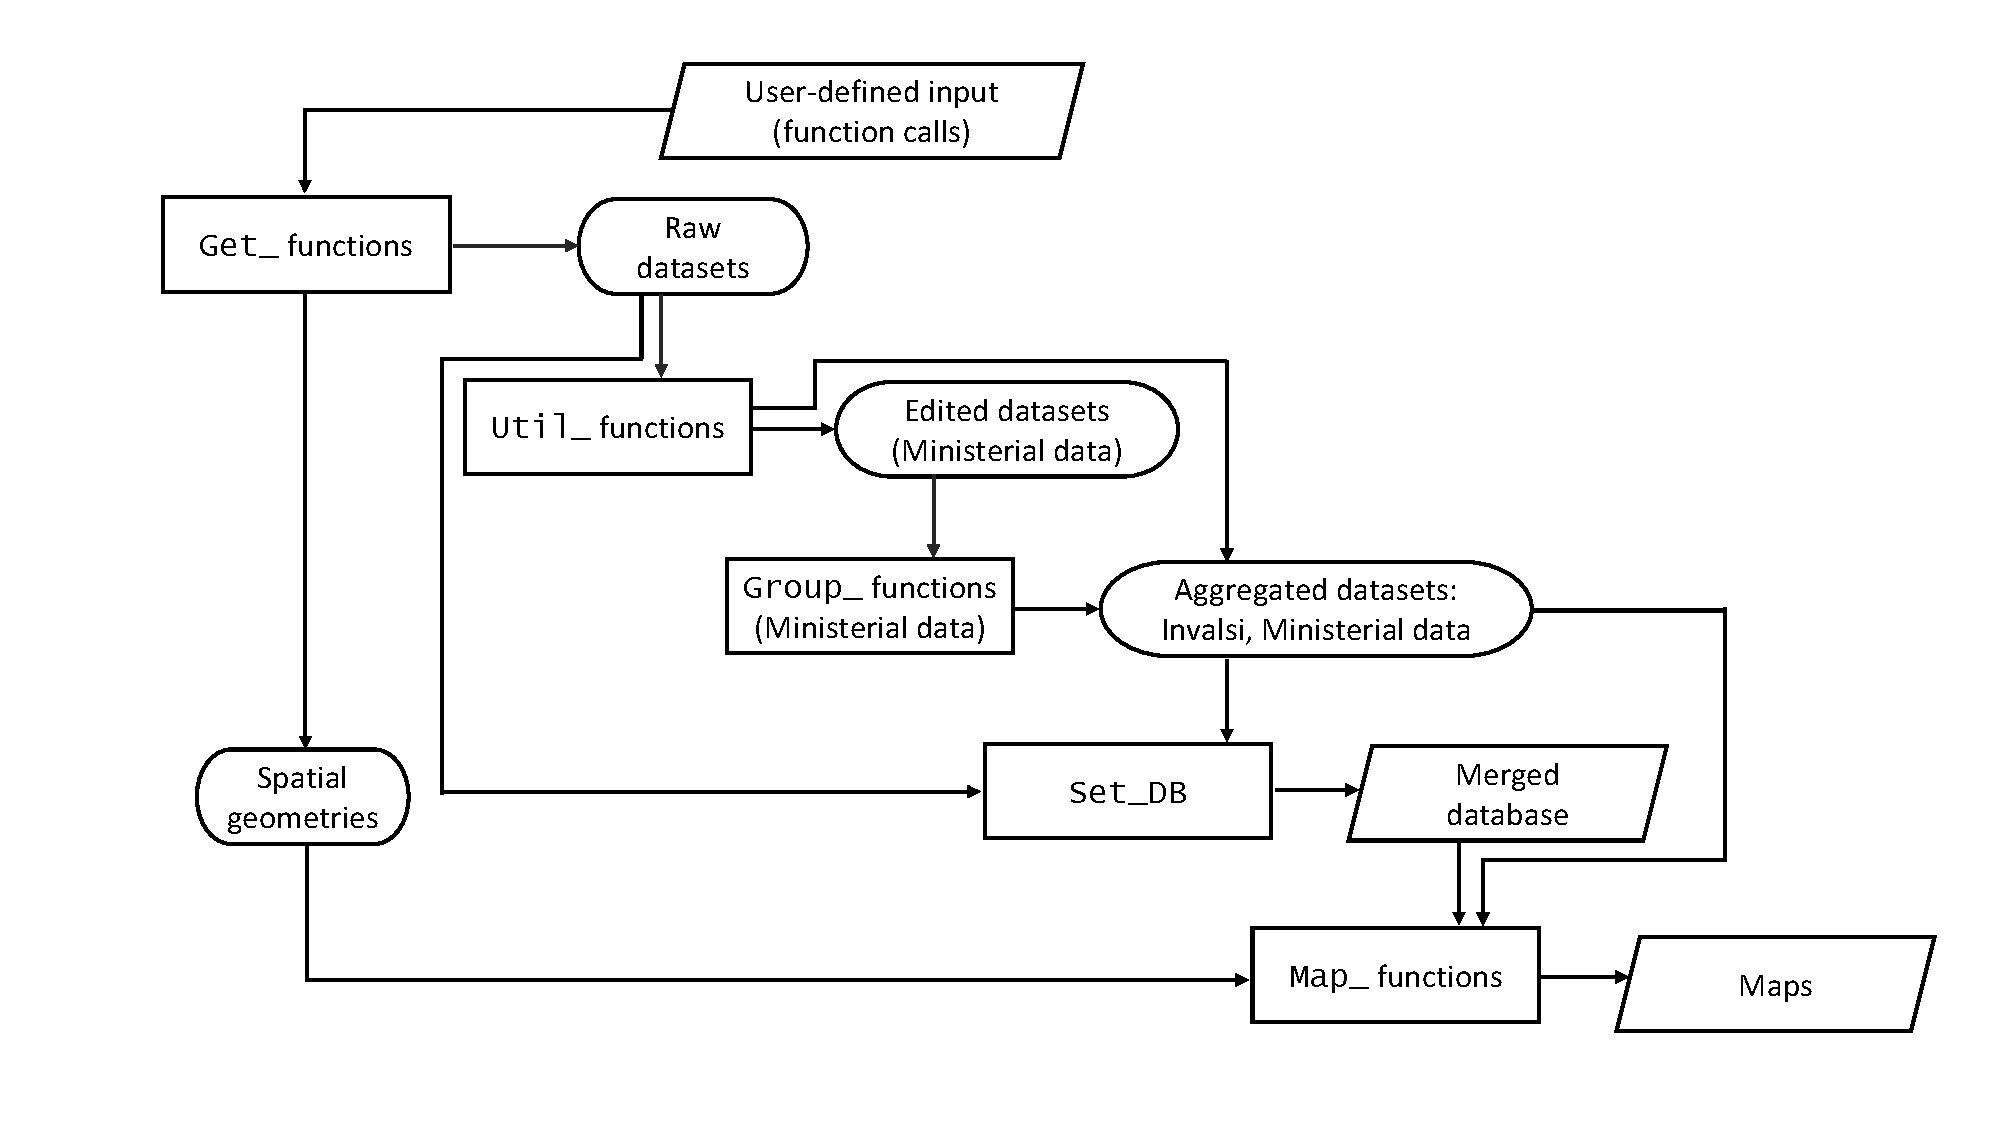
\includegraphics[width = 0.9\textwidth]{Fig1.pdf} 
  \caption{Flowchart of the package. Rhomboids denote inputs and \texttt{R} output objects; rectangles denote functions and rounded rectangles denote intermediate \texttt{R} objects.}
  \label{fig:Flowchart}
\end{figure}

The first step involves retrieving school system data from institutional sources through the \texttt{\detokenize{Get_}} functions. The user specifies some key requests in function calls, such as the school year of interest for school buildings or student counts data; then the software navigates to the webpage of the data provider and downloads the dataset in scope by HTML inspection. No storage space is required on the local machine of the user. The main retrieval functions are the following; reported data availability is assessed on April 3rd 2025.
\begin{itemize}
    \item \texttt{\detokenize{Get_DB_MIUR}} for school infrastructure data, available for school years 2015/16, 2017/18, 2018/19, 2020/21, 2021/22 and 2022/23;
    \item \texttt{\detokenize{Get_Invalsi_IS}} for Invalsi census data, available for school years from 2012/13 to 2023/24 except for 2019/2020; 
    \item \texttt{\detokenize{Get_nstud}} for student counts, available for school years 2015/16, 2017/18, 2018/19, 2020/21, 2021/22, 2022/23 and 2023/24;
    \item \texttt{\detokenize{Get_BroadBand}} for the activation status of the ultra-broadband connection across single schools at a user-specified date;
    \item \texttt{\detokenize{Get_nteachers_prov}} for teachers counts by province, available for the same school years as the school buildings data;
    \item \texttt{\detokenize{Get_Registry}} for the National Schools Registry, available for school years from 2015/16 to 2024/25;
    \item \texttt{\detokenize{Get_School2mun}} to map each school to the relevant administrative unit codes, available for the same years as the school buildings data.
\end{itemize}
The resulting objects are faithful to the original data published by providers, since at this stage data are not edited yet besides some manual corrections to municipality and province names needed for harmonising and mapping. 

Indeed, data manipulation is reserved for the subsequent step, namely the \texttt{\detokenize{Util_}} functions. One aim of these auxiliary functions is to transform input data into objects that can be handled with the next group of functions. The other aim is to perform data quality checks or editing. This group includes \texttt{\detokenize{Util_Check_nstud_availability}} to check how many schools have available the student counts, \texttt{\detokenize{Util_DB_MIUR_num}} to structure Boolean and numeric fields in the school buildings database or remove either observations with missing fields or fields with a given amount of missing observations, \texttt{\detokenize{Util_Invalsi_filter}} to filter the Invalsi survey for the school year, grade and subject, and \texttt{\detokenize{Util_nstud_wide}} to reshape the student counts dataset for it to have one school per row, compute average classroom size for each school grade, and filter out schools for which the classroom size is considered an outlier. Additional details on these functions are provided in Section \ref{sec:Data}. 

Ministerial data are provided at the school level. \texttt{\detokenize{Group_}} functions allow users to bring them to the same level of detail, namely at the LAU or NUTS-3 level. The function \texttt{\detokenize{Set_DB}} merges one or more datasets from the previous steps into a unique, aggregated database which can be considered as the final data output of the package workflow.

Lastly, the \texttt{\detokenize{Map_}} functions render aggregated data with static or dynamic choropleth maps. Notice that the former employs the \texttt{ggplot2} \citep{ggplot} environment for graphical representation, allowing a simplified export. Interactive maps, obtained through the \texttt{leaflet} \citep{leaflet} and \texttt{mapview} \citep{mapview} libraries, preserve all the information of the dataset to be rendered. Spatial geometries used for mapping are provided by the Italian Institute of Statistics through specific shape files \citep{Shapefiles}.

 

%%%%%%%%%%%%%%%%%%%%%%%%%%%%%%%%%%%%%%
%%%%%%%%%%%%%%%  Data  %%%%%%%%%%%%%%%
%%%%%%%%%%%%%%%%%%%%%%%%%%%%%%%%%%%%%%
\section{The Italian Education System Data} \label{sec:Data}
This section describes the main datasets currently retrieved and handled by the package. For the school infrastructure system evaluation, the most valuable public source of information is the Unique School Data Portal \citep{MIUR}, an open data portal managed by the Italian Ministry of Education according to Law 107/2015 \citep{law2}. The National Schools Registry (Section \ref{par:registry}), the school buildings database (\ref{par:buildings}) and the counts of students and teachers (\ref{par:nstud}) are all provided through this portal. Another relevant aspect of school infrastructure assessment is the implementation of ultra-broadband connection, whose timeline, available through the ultra-broadband activation dashboard, provided by \cite{BB} has been included in the package as well.
Lastly Invalsi censuary survey data \citep{Invalsi_IS} have been included to assess education quality (\ref{par:Invalsi}).

Italian schools are officially identified by a 10-digit alphanumeric code. In Fig. \ref{fig:diagram} we show an example of the identifiers (ID) hierarchy. The top node is the reference institute ID; intermediate nodes are the school institutes IDs; whereas bottom nodes are the school buildings IDs. For instance, under the same reference institute, two schools are located in the municipality of Casamassima (BA, code 72015) while five other ones are distributed across three buildings in the municipality of Acquaviva delle Fonti (BA, code 72001).
\begin{figure}
  \centering
  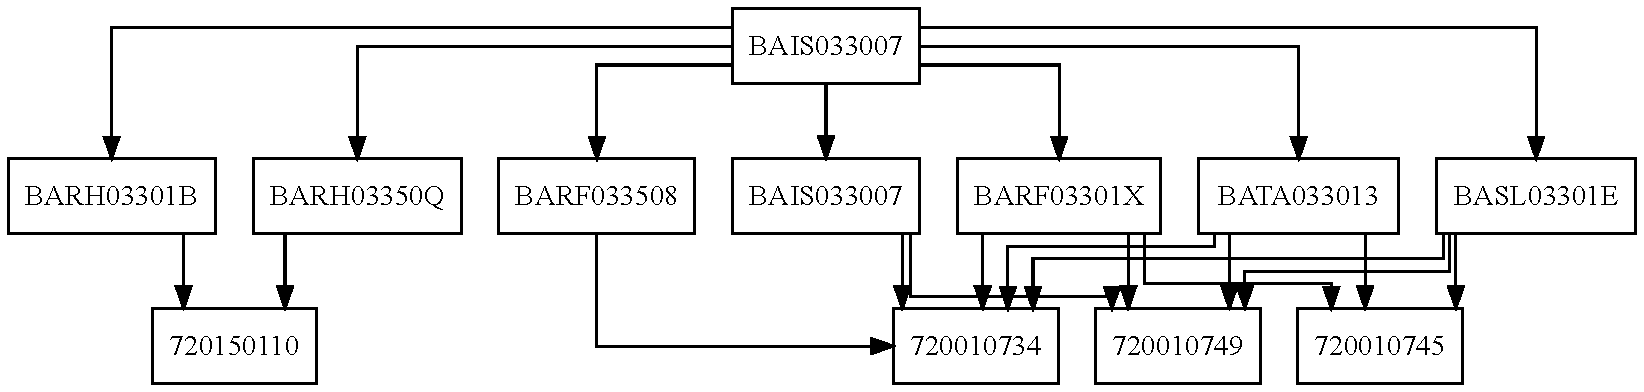
\includegraphics[width = 0.9\textwidth]{Fig2.pdf} 
  \caption{Example of the codes of all the schools (middle nodes) and the buildings in which they are located (bottom nodes), pertaining to the same reference institute (top node)}
  \label{fig:diagram}
\end{figure}

\subsection{National Schools Registry} \label{par:registry}
The National Schools Registry includes the list of all public and private schools on the national territory. Due to the completeness of the records, this dataset is used as the baseline to harmonise other objects defined at the school level. The function \texttt{\detokenize{Get_Registry}} downloads the dataset. Notice that the relevant municipality of each school is not identified by its official administrative code but only by the cadastral code. To fill this gap, the function \texttt{\detokenize{Get_School2mun}} associates each school listed in this registry with the relevant administrative (LAU and NUTS-3) codes \citep{Situas}.

\subsection{School Buildings} \label{par:buildings}
This database covers several infrastructural dimensions, accounting for a total of about 90 variables in the last available year:
\begin{itemize}
 \item Environmental context of school buildings
 \item Accessibility through private or public transport, namely whether a building lies within a given range (e.g. 250 or 500 meters) from a transport hub
 \item Environmental or administrative restrictions 
 \item School area surface and building volume
 \item Intended use of learning and recreational spaces
 \item Overcoming architectural barriers (e.g. the presence of external ramps or stairlifts)
 \item Building and adaptation period
 \item Various information regarding heating systems
 \item Measures and devices to reduce energy consumption
 \item Acoustic insulation
 \item Static testing certification and seismic design
\end{itemize}
Observations are detailed at the level of school buildings. For this reason, the database embeds a standalone registry different from the National Schools Registry mentioned in the previous paragraph. %School years covered are 2015/16, 2017/18, 2018/19, 2020/21, 2021/22 and 2022/23.

The input dataset downloaded with \texttt{\detokenize{Get_DB_MIUR}} includes about $60,000$ observational units. Most variables are binary (Y/N), denoting whether a given feature occurs in a school building or not, and encoded as strings.

The function \texttt{\detokenize{Util_DB_MIUR_num}} converts strings to Boolean or numeric values when necessary. For some variables, there is a high number of missing values. For example, in school year 2022/23, the field denoting whether a school is reached by a bicycle lane is missing for $38.7\%$ of high schools, $44.1 \%$ of primary and $45.9\%$ of middle schools. The user may choose to remove either the fields with a given number of missing records ($20,000$ by default) or the units with at least one missing variable (not active by default). 

Observations can be aggregated with the function \texttt{\detokenize{Group_DB_MIUR}}. Numeric and Boolean variables are summarized by their mean and qualitative variables by their mode. Since territorial averages provide no information about missing values, by default the function returns two additional data frames providing the number of missing observations of each variable per area.

Finally, for better insight into the general infrastructural state, we add the Inner Areas taxonomy, published by the Italian Institute of Statistics (ISTAT) and updated every six years \citep{InnerAreas}. It divides Italian municipalities into six classes: A, B and C are considered central areas, while D, E, and F classes are labeled as "inner" (i.e. peripheral) areas. Class A identifies standalone pole municipalities, characterized by a comprehensive and self-sufficient combination of school, health, and transport infrastructure \citep{InnerAreas}; class B identifies inter-municipality poles, i.e. clusters of neighbouring municipalities which, taken together, fulfill the requirements of pole municipalities. The remaining classes are defined based on increasing road travel time to the closest pole: Class C: $0' - 27'42''$; Class D: $27'42'' - 40'54''$; Class E: $40'54'' - 1h \, 6' 54''$; Class F: $> 1h \, 6' 54''$.

In Figure \ref{fig:TPU23} we show the percentage of schools served by public transport in 2022/23 at the province and municipality level, in this latter case only for the Apulia region, which is the region with the highest share of municipalities hosting at least one high school ($124$ over $257$). As mentioned in Section \ref{sec:Data}, though northern and central regions have a higher proportion of schools served by urban public transport, regions like Abruzzo in the South or Veneto and Emilia-Romagna in the North are in contrast the general trend. In the provinces of Aosta, Trieste, La Spezia (North), Massa (Center) and Chieti (South) all schools are reached by public transport, while this percentage is higher than $95\%$ in the provinces of Pavia, Bergamo (North), Pesaro-Urbino, Pisa, Lucca and Latina (Center). On the other hand, in the province of Salerno in Southern Italy only $0.07\%$ of schools is served by public transport; this percentage is lower than $40\%$ in the provinces of Ferrara and Pordenone in the North and Crotone, Foggia and Naples in the South.%The negative record belongs to the provinces of Salerno and Naples in Campania and Crotone in Calabria.

The code to download the raw input dataset and display these maps and all the following ones is in the Supplementary Material. 

\begin{figure}
  \centering
  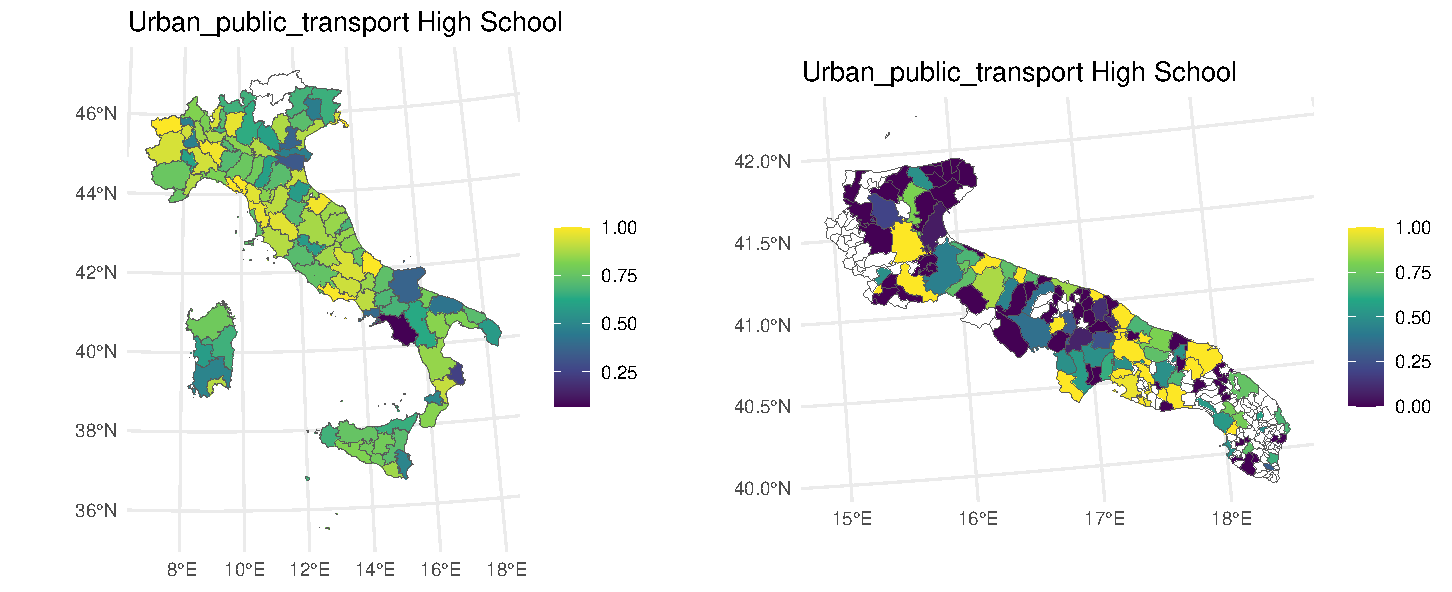
\includegraphics[width = 0.9\textwidth]{Fig3.pdf}  
  \caption{Province-level and municipality-level percentage of high schools served by public transport in 2022/23, on the whole national territory and in the Apulia region respectively. Data of the Trentino-Alto Adige region are not provided by the Ministry.}
  \label{fig:TPU23}
\end{figure}

\subsection{Number of students and teachers} \label{par:nstud}
The Ministry of Education also publishes the counts of students per school grade for every school on the Italian territory and the counts of teachers for every Italian province. These datasets have the same temporal dimension as the school buildings database. classroom size is indeed useful information in the assessment of education quality, which is typically acknowledged to improve as classroom size decreases \citep{Blatchford, Bruhwiler}. In the case of Italy, however, caution is needed when studying the relationship between classroom size and student outcomes at the aggregate level \citep{Angrist}. In our view, an important factor to consider is how classroom size reflects the degree of centrality of municipalities. As it can be seen in Figure \ref{fig:nstud_bp_8} as an example for the last year of middle schools, peripheral areas, usually characterized by lower student outcomes, have less crowded classrooms. We will have a deeper look at the association between classroom size and education quality in Section \ref{sec:Example}.
\begin{figure}
  \centering
  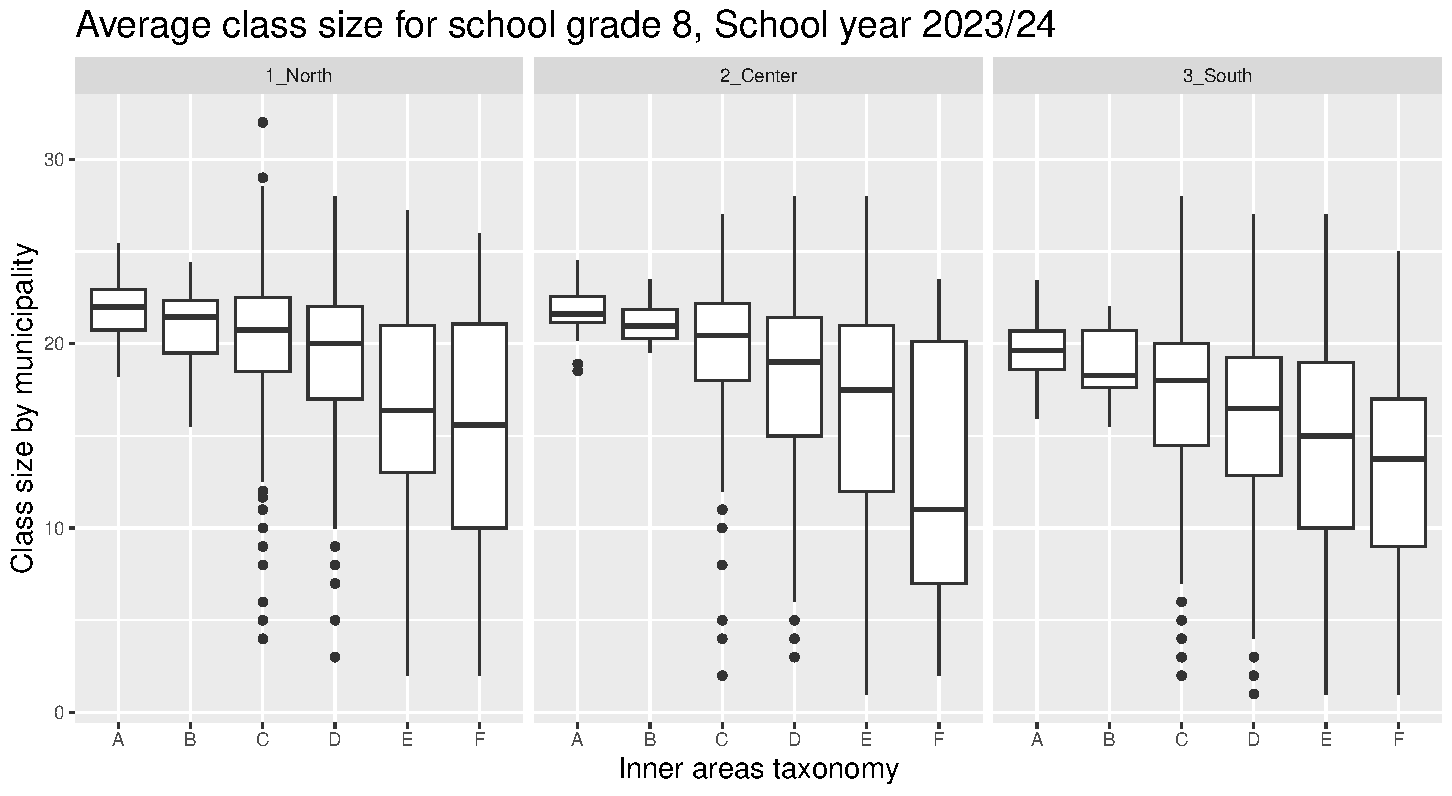
\includegraphics[width = 0.9\textwidth]{Fig4.pdf} 
  \caption{Average municipality-level classroom size by Inner Areas taxonomy in 2023/24, last grade of middle schools. Inner area taxonomy follows a descending order of centrality: A - standalone infrastructural poles; B - inter-municipality infrastructural poles; C - belt municipalities; D - intermediate areas; E - peripheral; F - ultra-peripheral.}
  \label{fig:nstud_bp_8}
\end{figure}


The function \texttt{\detokenize{Util_nstud_wide}} rearranges the input dataset into a wide format in which each row corresponds to a school and computes the average classroom size per school for each educational grade. National regulation sets upper classroom size limits of $25$, $26$ or $27$ students in primary, middle and high schools respectively \citep[][Art. 5]{DMIM90} other than lower limits of $15$ students (8 for multi-year classes) in primary schools and $18$ students in middle schools through the Decree n.90/2023 of the Ministry of Education \citep[][Artt 10, 11]{DPR81}. A framework of waivers is established by the Ministry Decree n.90/2023 \citep{DPR81}, regarding cases of low Economic, Social and Cultural Status (ESCS) scores, high school withdrawal rate or high depopulation. 
However, the range of observed classroom sizes is often wider than the general rule, especially in high schools. In the latter case, taking the school year 2022/23 as an example, the number of schools with classroom size $\geq 40$ students was equal to $9$, $8$, $8$, $18$ and $1$ for the five high school grades respectively, over a total of $6455$ schools.
To remove values considered extreme, the user can set an upper and a lower boundary of acceptance in terms of classroom size either at the level of whole schools or single school grades. In the former case, only schools whose average classroom size (computed across all grades, e.g. for middle schools the average of 6th, 7th and 8th grades) exceeds the acceptance boundary are removed from the dataset, while in the latter case removal applies to all schools where classroom size exceeds the boundary in any grade.
For what concerns primary schools, it is also possible to download student counts by type of schooling time, namely distinguishing between full-time and half-time (only morning) schooling.

To monitor statistical data quality, the function \texttt{\detokenize{Util_nstud_check}} computes, for all municipalities and provinces, the percentage of schools listed in the National Registry for which the count of students is available. 

The function to aggregate school-level data is \texttt{\detokenize{Group_nstud}}.

Teacher counts, instead, are only available at the province level. The average number of teachers per student and per class can be computed with the function \texttt{\detokenize{Group_nteachers4stud}}. In Figure \ref{fig:nstud23} we render the average classroom size in the 2nd year of high school and the average number of teachers by student in the year 2022/2023. classroom size is higher in densely populated areas, such as the Po Valley and the surroundings of Rome and Naples, while it is smaller in most of the South, especially in the Apennines and in Sardinia. The teacher/student ratio follows a similar distribution.

\begin{figure}
  \centering
  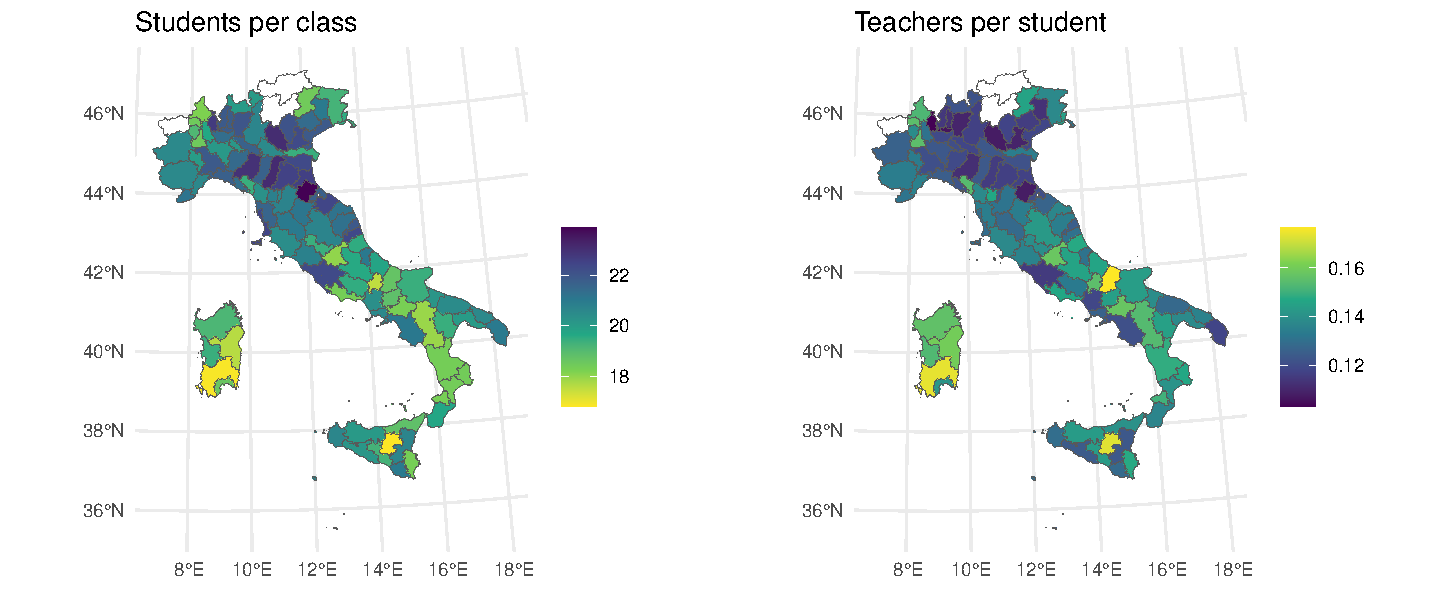
\includegraphics[width = 0.9\textwidth]{Fig5.pdf} 
  \caption{Average province-level classroom size in the 2nd year of high school and province-level teachers/students ratio in high schools in 2022/23. Data are not available for the Trentino-Alto Adige and Aosta Valley regions. Additionally, schools with average classroom size of less than $10$ or more than $40$ students in any grade have been filtered out. }
  \label{fig:nstud23}
\end{figure}

\subsection{Ultra - Broadband connection in schools} \label{par:BB}
This dataset consists of the list of schools of the National Ultra-Broadband Plan, approved by the Ministry of Economic Development with the decree of 07/07/2020 \citep{law3}. The Plan aims at providing 32.164 schools with internet connection with a maximum speed of 1 gigabit/second and a symmetric minimum guaranteed speed of 100 megabits/second until the peering is reached. Data are updated monthly \citep{BB}. In Table \ref{tab:broadband} in the \ref{Appendix1} we show the number of schools in which the ultra-broadband was activated in different years for all regions (one school in Trentino Alto Adige had a broadband connection before 2020). The function to download this dataset is \texttt{\detokenize{Get_BroadBand}}; the \texttt{Date} argument specifies the reference date for checking whether the ultra-broadband connection was activated or not in each school. 

\subsection{Invalsi census survey} \label{par:Invalsi}
To develop a spatially homogeneous indicator of education quality, Italian law No. 176/2007 \citep{law} mandates the Italian Institute for the Evaluation of the Education System (INValSi) to assess the skills of students through a specific test. The test currently covers four subjects, Italian, Mathematics, English reading, and English listening, and is carried out yearly in the 2nd, 5th, 8th, 10th, and 13th school grades. 
The Invalsi Institute publishes several open datasets \citep{Invalsi_IS}, the widest class being that of sample surveys, which also includes anonymized microdata regarding single students. The other class of datasets consists of census surveys, detailed at either municipalities or provinces. Regarding municipality data, for privacy reasons only the municipalities with at least two schools of the same order are included in the survey; otherwise identifying average Invalsi scores of single schools would be easily possible. In this package, we focus on the census dataset since it provides more spatial information (sample datasets providing no territorial information other than the region) and is, in our judgment, more suitable for spatial analysis. 
%Census data for territorial aggregates are available for every school year from 2012/13 to 2023/24, except for 2019/2020. 
Consistently with OECD standards \citep{PISA} the score is expressed through the weighted likelihood estimator (WLE) of student ability defined by a Rasch psychometric model, whose basic idea is that the probability that a generic student $i$ answers correctly to a generic item $j$ (i.e. to a generic test question) depends on two variables, namely the student ability $b_i$ and the item difficulty $d_j$. The relationship can be expressed as
$$
\mathrm{Prob} \lbrace \text{student } i \text{ answers correctly item } j \rbrace= \frac{e^{b_i - d_j}}{1 + e^{b_i - d_j}}
$$
For interpretational reasons, the estimator of $b_j$ is scaled to a global mean of 200 points and a global between-students standard deviation of 40 points. The advantage of this model is isolating the ability of students from the intrinsic difficulty of items. For primary schools only, the percentage of sufficient tests is also reported. Scores are already corrected from the effect of cheating, which would otherwise hinder their meaning, other than shrinking their variance. The functions to download and filter the Invalsi database per school year, grade and subject are respectively \texttt{\detokenize{Get_Invalsi_IS}} and \texttt{\detokenize{Util_Invalsi_filter}}. No data quality checks are deemed necessary as this dataset is already carefully processed by the Invalsi Institute.

As an example, in Figure \ref{fig:Invalsi} we plot the Invalsi scores in Italian and English reading for the last year of high school at the province level in 2023/24. The North-South divide is obvious. A particularly vulnerable profile can be noticed across the provinces of Naples and Salerno (Campania) and most of the provinces belonging to Calabria, Sicily, and Sardinia (with the partial exception of the province of Cagliari). Highest scores in both subjects are observed in the provinces of Lecco, Como and Bergamo in Lombardy other than Trieste and Bolzano with respect to English scores.

\begin{figure}
  \centering
  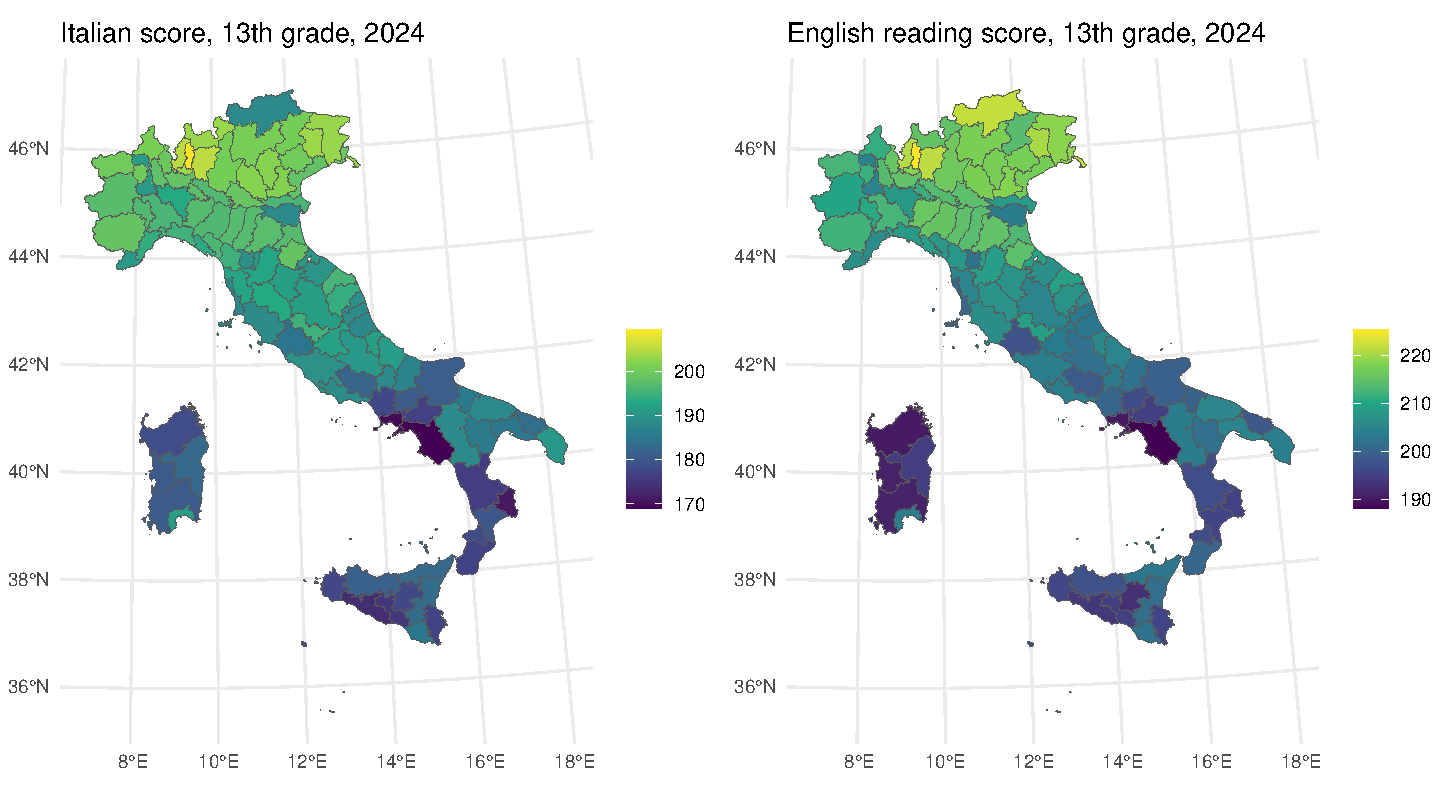
\includegraphics[width = 0.9\textwidth]{Fig6.pdf} 
  \caption{Invalsi scores in Italian and English reading, last year of high school, school year 2023/24}
  \label{fig:Invalsi}
\end{figure}





%%%%%%%%%%%%%%%%%%%%%%%%%%%%%%%%%%%%%%%
%%%%%%%%%%%%%%% Example %%%%%%%%%%%%%%%
%%%%%%%%%%%%%%%%%%%%%%%%%%%%%%%%%%%%%%%
\section{Student outcomes in Mathematics and classroom size: an example using the SchoolDataIT package} \label{sec:Example}

Here we provide an example of spatial statistical application to the data covered by the \texttt{SchoolDataIT} package. Following Section \ref{par:nstud}, suppose the user is interested in studying to what extent classroom size is associated with student outcomes. We can first map the two variables.
%
\begin{figure}
  \centering
  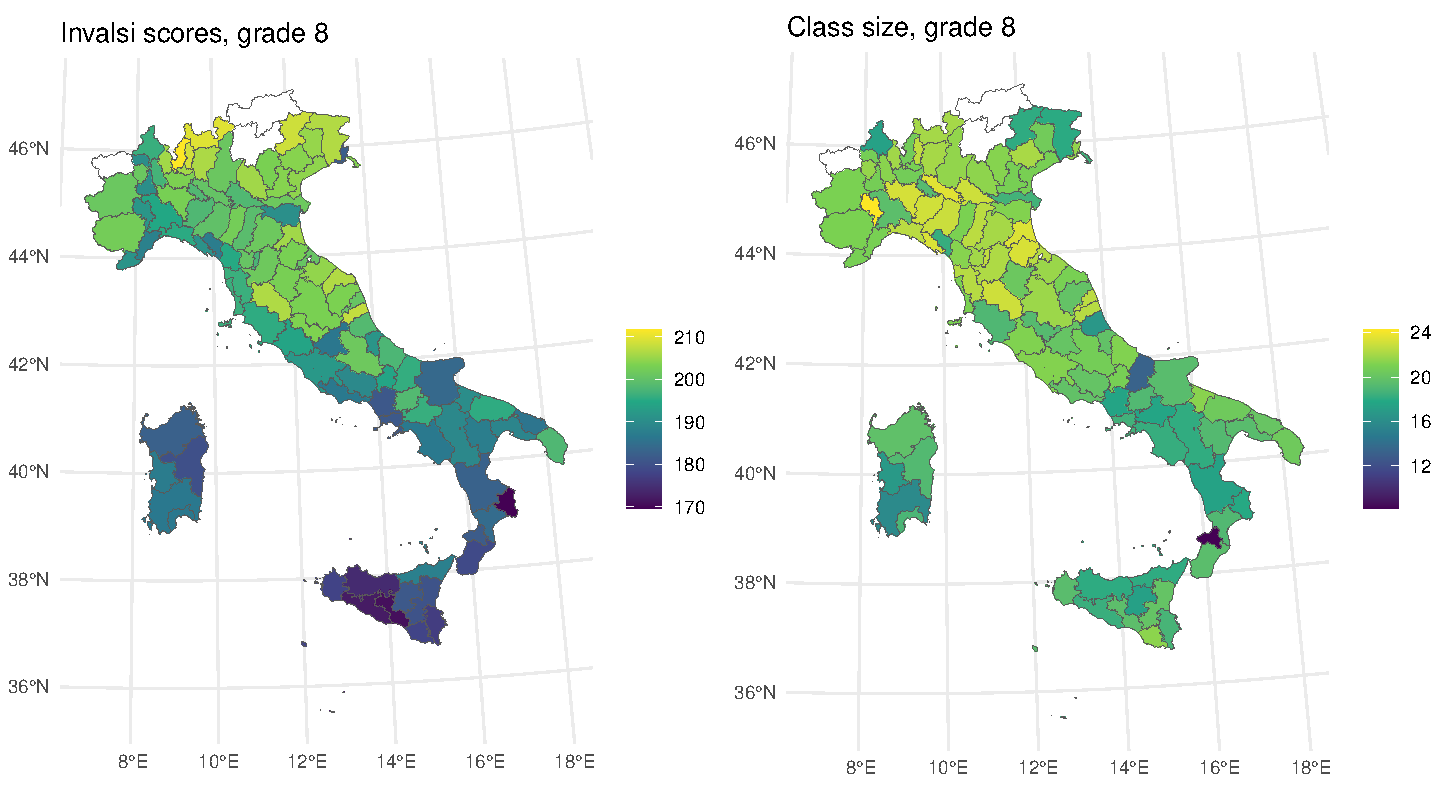
\includegraphics[width = 0.9\textwidth]{Fig7.pdf} 
  \caption{Invalsi score in Mathematics and average classroom size, last year of middle school, school year 2023/24. Trentino-Alto Adige and Aosta Valley are not included due to lack of classroom size data.}
  \label{fig:invalsi_nstud8}
\end{figure}
%
Concerning the last year of middle school in 2023/2024, we regress the Invalsi score in Mathematics on the average classroom size at the municipality level. To ease model results interpretation, classroom size is scaled to zero mean and unit variance. Additionally, schools with an average class size of less than $10$ or more than $40$ students have been removed from the dataset. 
In this case, observational length is equal to $n = 780$ municipalities, i.e. those for which Invalsi scores and classroom size were both available at 2025/04/03.

OLS regression would result in an expected effect of classroom size equal to $4.153$, with standard error $0.407$. If no additional information is taken into account, classroom size would then appear to have a positive and statistically significant relationship with Invalsi scores.
%Under the OLS specification, the stochastic representation of the Invalsi score, which we denote as $y$, is
%%
%\begin{equation}
%y = \beta_0 +  \beta_\mathrm{nstud} X_\mathrm{nstud} + \varepsilon
%\label{eq:OLS}
%\end{equation}
%%
%where $\beta_0$ is the intercept, $X_\mathrm{nstud}$ is classroom size, $\beta_\mathrm{nstud}$ is the effect of classroom size, and $\varepsilon$ is a Gaussian IID error such that $\varepsilon \sim N  (0, \sigma_{\varepsilon}^2 I_n)$. 

%If no additional information is taken into account, classroom size appears to have a positive and statistically significant association with the Invalsi score, as seen in \ref{tab:OLS}:
%
% \begin{table}
% \centering
%\begin{tabular}{lrrrr}
% & mean & s.d. & $Q_{0.025}$ & $Q_{0.975}$ \\
% \hline
% $\beta_0$ (intercept)& 194.551 & 0.406 & 193.755 & 195.347 \\ 
% $\beta_{nstud}$ & 4.153 & 0.407 & 3.356 & 4.951 \\ 
% \hline
%\end{tabular}
%\caption{Effect of classroom size on Invalsi scores in Mathematics in the last year %of middle school, using the model in eq. \ref{eq:OLS}}
%\label{tab:OLS}
%\end{table}
%
A closely linked result, namely the significantly positive association of Invalsi scores with the students/teacher ratio, was noticed by \cite{Barbieri}, always in the context of middle schools, and attributed to the impact of schools reputation on their attractiveness. Interestingly, when an instrumental variable relating to teachers' mobility was taken into account in their regression model, the estimated effect of the student-to-teacher ratio was not significant anymore.

Given the greater amount of information at our disposal, it would be na{\"i}ve to limit the analysis to this amount of information. First, considering what we have seen in \ref{fig:nstud_bp_8}, the user may be interested in adding the inner areas taxonomy as an explanatory variable in the simplest possible way, namely classifying municipalities among central (A, B, C) and inner (C, D, E) areas. Moreover, the territorial structure of the dataset suggests to include spatial terms in the regression model. Considering the number of municipalities for which data are available ($780$ over a national total of $7901$), the spatial structure is rather sparse and we would need to define some neighbouring rules in alternative to shared borders. To overcome this issue, we choose to treat the municipality-level average Invalsi score as a point-referenced process, thus assuming that the data-generating process is defined on a continuous spatial domain. Specifically, we postulate that the locations at which this process is observed are the centroids of municipalities as defined on January 1st, 2023.
Spatial information is taken into account through a linear spatial trend and a spatially structured Gaussian process $u$ whose autocorrelation decays as distance increases. The model becomes thus:
%
\begin{equation}
y = \beta_0 + \beta_\mathrm{nstud} X_\mathrm{nstud} + \beta_{I} X_{I} + \beta_{\ell} \ell +\beta_{\phi} \phi + u + \varepsilon
\label{eq:spde}
\end{equation}
%
where $\beta_0$ is the intercept, $X_\mathrm{nstud}$ is classroom size, $X_I$ is the dummy for the inner areas taxonomy ($1$: inner area, $0$: central area), $\ell$ is the longitude of municipality centroids, $\phi$ is the latitude; $\beta$ terms are covariates effects; $\varepsilon$ is a Gaussian IID error such that $\varepsilon \sim N  (0, \sigma_{\varepsilon}^2 I_n)$. $u$ follows \textit{a priori} a Normal distribution with mean zero and covariance matrix whose elements depend on the distance between the two corresponding points, but not on the direction of their link (isotropy); second-order stationarity is additionally assumed for $u$ \citep[][ Section 2.1]{Banerjee}. Based on these two assumptions, we assign $u$ the Matérn covariance function, which depends on a global variance $\sigma^2$ and a range parameter $r$; details on the Matérn covariance are in Appendix \ref{subsection:Matern} and information on model computation is in Appendix \ref{subsection:SPDE}.

The hierarchical model in equation \ref{eq:spde} also requires prior assumptions on the distribution of its hyperparameters. Error precision $\sigma_{\varepsilon}^{-2}$ is assumed to follow a Gamma distribution with shape parameter $1$ and rate parameter $ 5 \cdot 10^{-5}$. Moreover, we define a penalized complexity (PC) prior \citep{PC} on the range $r$ and the global standard deviation $\sigma$ of the latent spatial field. The behaviour of these distributions is described in \cite{SPDEPC}. We select two fixed values, $\sigma_0$ and $r_0$ such that, for two fixed values $p_\sigma$ and $p_r$, $prob \left( r < r_0 \right) = p_r $ and $prob \left( \sigma > \sigma_0 \right) = p_\sigma$. 

Based on prior knowledge and ignoring the information available from exploratory data analysis, we assume that the range, namely the distance at which the correlation of the random fields is shrunk under a $0.10$ threshold, is smaller than $300$ kilometers with $5\%$ probability, and the standard deviation of the random field is higher than $4$ points with $5\%$ probability. Again, for the sake of model results interpretation, classroom size, latitude and longitude are scaled to mean $0$ and variance $1$. 

The summaries of covariate effects are reported in Table \ref{tab:betaSP}.
%
 \begin{table}
 \centering
\begin{tabular}{lrrrr}
 & mean & s.d. & $Q_{0.025}$ & $Q_{0.975}$ \\
 \hline
 $\beta_0$ (Intercept) & 195.103 & 1.080 & 192.918 & 197.211 \\  
 $\beta_{nstud}$ 0.192 & 0.317 & -0.429 & 0.813 \\ 
 $\beta_I$ & -2.329 & 0.719 & -3.743 & -0.920 \\ 
 $\beta_{\phi}$ & 8.997 & 1.044 & 6.928 & 11.061 \\ 
 $\beta_{\ell}$ &  1.865 & 1.038 & -0.174 & 3.934 \\ 
 \hline
\end{tabular}
\caption{Estimated effects of classroom size, inner area dummy, latitude and longitude on Invalsi scores in Italian, last year of middle school, under model \ref{eq:spde}}
\label{tab:betaSP}
\end{table}
%
Employing this amount of information, the effect of classroom size no longer appears to be significant, while belonging to an inner area still implies an expected disadvantage of $2.329 $ points in Invalsi scores compared to central areas (either infrastructural poles or municipalities close to them). The evidence for the North-South divide is very strong, as the current model suggests that being located one standard deviation of the northing distribution ($\approx 291.25$ km) further north than a reference location implies an expected advantage of $8.997$ Invalsi points. To visualize the extent to which the spatial structure influences Invalsi scores, we plot the expected value of the linear trend ($\beta_\ell \ell + \beta_\phi \phi$) and the latent Gaussian process ($u$) in Figure \ref{fig:trends}.

The darker zones in the right panel (lower values of $\mathbf{E}[u|y]$) can be interpreted as areas of educational vulnerability net of classroom size, general infrastructural conditions, and net of the North-South trend as well. Most critical areas include the urban area of Naples and the upper Ionian coast in Calabria. Conversely, brighter areas represent relatively advantaged territories, such as much of  Central inland and the Salento Peninsula.
% The most critical areas include the Po Delta (between Emilia-Romagna and Veneto), the Gargano peninsula (Apulia), the urban area of Naples, the upper Ionian coast in Calabria, and Northwestern Sardinia. Conversely, brighter zones represent relatively advantaged territories, such as the Nebrodi mountains and the province of Enna (Sicily), the Salento peninsula (Apulia), and much of inland Central Italy.
\begin{figure}
  \centering
  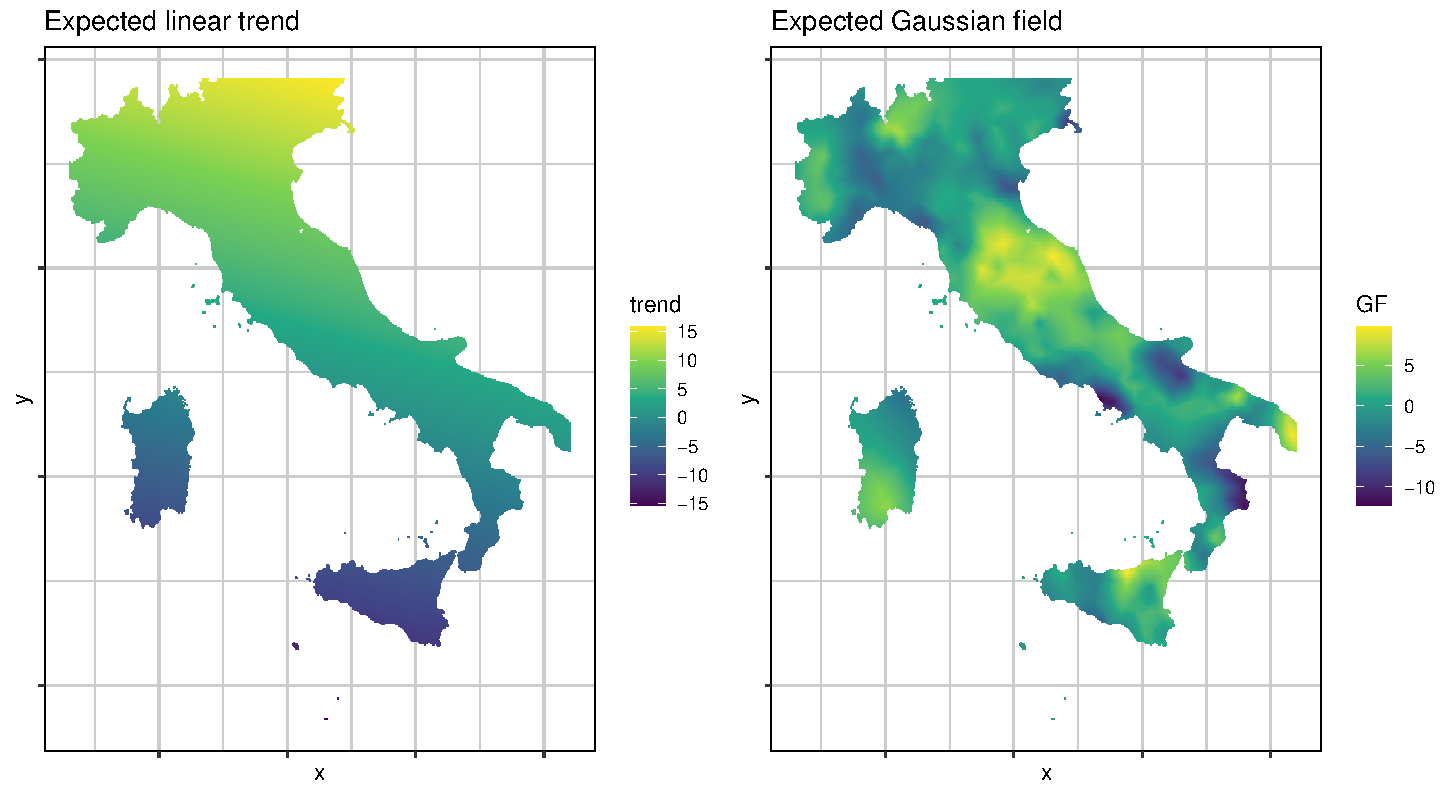
\includegraphics[width = 0.9\textwidth]{Fig8.pdf} 
  \caption{Posterior expectation of the linear trend on the left and of the spatial latent variable on the right, the latter being added to the model to explain spatial variability in Invalsi scores after controlling for the linear trend and the explanatory variables.}
  \label{fig:trends}
\end{figure}


This simple example highlights that assessing the impact of classroom size on student outcomes is somewhat less simple than it may initially appear and warrants a multidimensional analysis. Even though only aggregated data are taken into account, auxiliary information such as the degree of centrality of a municipality or the spatial location becomes thus crucial.





%%%%%%%%%%%%%%%%%%%%%%%%%%%%%%%%%%%%%%%%%%%
%%%%%%%%%%%%%%% Conclusions %%%%%%%%%%%%%%%
%%%%%%%%%%%%%%%%%%%%%%%%%%%%%%%%%%%%%%%%%%%
\section{Concluding remarks}
The package \texttt{SchoolDataIT} allows \texttt{R} users to automatically construct an organic database by combining from different sources those open data we deem to be the most informative about the Italian education system and the state of school infrastructure in Italy, covering some of the Ministerial open data sets (e.g., the Schools Registry, the school buildings database, students and teachers counts), the Invalsi census survey, and the registry of Ultra-Broadband activation status. 

One key feature we emphasize is the relevance of the spatial context, hence territorial units of aggregated data can be easily associated either with their boundaries or centroids. With this library, we aim to provide an insight into the state of the Italian education system as clearly as possible, to ease statistical analysis on its main aspects, also employing a spatial framework, and to identify areas of education vulnerability following either a unidimensional or a multidimensional approach. With this in mind, exploratory analysis should be facilitated by mapping functions. While this paper presents a cross-sectional data usage example, panel analysis is possible as well, considering a current observation length of six years. 

Although the present version of the package covers a given amount of data, implementing any additional function to retrieve, edit and structure further data sets would not imply a significant increase in file weight for the package. Therefore, a possible line of development of this package would be to plug in additional data sets.

Lastly, the package appeals to generic \texttt{R} users, from whom the various functions are designed to require as little effort as possible. Despite our efforts for maintaining a user-friendly perspective, the final output of this package is data objects defined coherently with the \texttt{Tidyverse} environment to ensure object portability and ease of use of the present data also outside \texttt{R}.



%%%%%%%%%%%%%%%%%%%%%%%%%%%%%%%%%%%%%%%%%%%%
%%%%%%%%%%%%%%% Bibliography %%%%%%%%%%%%%%%
%%%%%%%%%%%%%%%%%%%%%%%%%%%%%%%%%%%%%%%%%%%%
%
\bibliographystyle{apalike}
\bibliography{SchoolDataIT_References}
%
%
%
%

%%%%%%%%%%%%%%%%%%%%%%%%%%%%%%%%%%%%%%%%
%%%%%%%%%%%%%%% Appendix %%%%%%%%%%%%%%%
%%%%%%%%%%%%%%%%%%%%%%%%%%%%%%%%%%%%%%%%
\newpage
%\appendix
\begin{appendices} 

%\begin{table}[ht]
%\resizebox{\textwidth}{!}{% use resizebox with textwidth
%\centering
%\begin{tabular}{lrrrrrrrrrrrr}
%  \hline
%  Model \ Station & 60410 & 60430 & 60434 & 60512 & 61104 & 61402 & 61502 & 61603 & 62601 & 63001 & 65001 & 65101 \\ 
%   \hline
%\end{tabular}
%}
%\caption{Station-specific}
%\label{Tab:RelMSE}
%\end{table}

\section{Tables} \label{Appendix1}
\begin{table}[ht]
\centering
%\begin{scriptsize}
\resizebox{\textwidth}{!}{
\begin{tabular}{lrrrrrr}
  \hline
   & \multicolumn{2}{c}{Primary}& \multicolumn{2}{c}{Middle}& \multicolumn{2}{c}{High}\\
  Seismicity & buildings & \% tot. & buildings & \% tot. & buildings & \% tot. \\ 
  \hline
  High     & 1375 & 7.53\%  & 877  & 8.45\%  & 662  & 6.1\% \\ 
  Mid-High & 6999 & 38.33\% & 3938 & 37.96\% & 4267 & 39.31\% \\ 
  Mid-Low  & 7197 & 39.42\% & 3970 & 38.27\% & 4402 & 40.55\% \\ 
  Low      & 2687 & 14.72\% & 1589 & 15.32\% & 1524 & 14.04\% \\ 
   \hline
\end{tabular}
}
%\end{scriptsize}
\caption{Seismic risk classification of municipalities hosting school buildings}
\label{tab:seismicity}
\end{table}

%%%%%%%%%%%%%%%%%%%%%%%%%%%%%%%%%%%%%%%%%%%%%%%%%%%%%%%%%%%%%%%%%%%%%%%%%%%%%%%%%




\begin{table}[ht]
\centering
%\begin{scriptsize}
\resizebox{\textwidth}{!}{
\begin{tabular}{lrrrrrr}
  \hline
   & \multicolumn{2}{c}{Primary}& \multicolumn{2}{c}{Middle}& \multicolumn{2}{c}{High}\\
  Region & buildings & \% tot. & buildings & \% tot. & buildings & \% tot. \\ 
  \hline
  Abruzzo &  87 & 19.46\% &  62 & 22.46\% &  40 & 17.24\% \\ 
  Basilicata &  99 & 39.76\% &  73 & 40.33\% &  61 & 33.7\% \\ 
  Calabria & 608 & 60.5\% & 399 & 60.73\% & 234 & 52.58\% \\ 
  Campania & 191 & 10.43\% & 140 & 13.17\% & 143 & 12.25\% \\ 
  Emilia - Romagna &   1 & 0.09\% &   1 & 0.16\% &   0 & 0\% \\ 
  Friuli - Venezia Giulia &  42 & 8.47\% &  24 & 10.04\% &  16 & 6.3\% \\ 
  Lazio &  67 & 4.87\% &  34 & 4.32\% &  28 & 3.16\% \\ 
  Liguria &   0 & 0\% &   0 & 0\% &   0 & 0\% \\ 
  Lombardia &   1 & 0.04\% &   0 & 0\% &   0 & 0\% \\ 
  Marche &   2 & 0.38\% &   2 & 0.67\% &   0 & 0\% \\ 
  Molise &  40 & 30.3\% &  23 & 25.27\% &  21 & 22.11\% \\ 
  Piedmont &   0 & 0\% &   0 & 0\% &   0 & 0\% \\ 
  Apulia &  16 & 1.65\% &  14 & 2.34\% &  11 & 1.19\% \\ 
  Sardinia &   1 & 0.16\% &   2 & 0.41\% &   0 & 0\% \\ 
  Sicily & 131 & 7.78\% &  60 & 6.47\% &  48 & 4.75\% \\ 
  Tuscany &   0 & 0\% &   0 & 0\% &   0 & 0\% \\ 
  Umbria &  52 & 14.44\% &  25 & 12.69\% &  36 & 20.11\% \\ 
  Aosta Valley &   0 & 0\% &   0 & 0\% &   0 & 0\% \\ 
  Veneto &  37 & 2.26\% &  18 & 2.05\% &  24 & 2.97\% \\ 
  
   \hline
\end{tabular}
}
%\end{scriptsize}
\caption{School buildings located in high seismicity municipalities, both in absolute numbers and as a proportion of the regional total}
\label{tab:risk1}
\end{table}



%%%%%%%%%%%%%%%%%%%%%%%%%%%%%%%%%%%%%%%%%%%%%%%%%%%%%%%%%%%%%%%%%%%%%%%%%%%%%%%%%


%\begin{table}[ht]
%\centering
%\resizebox{\textwidth}{!}{
%\begin{tabular}{llllllllll}
%  \hline
% & \multicolumn{3}{c}{Seismic design}  & \multicolumn{3}{c}{Seismic adaptation}  & \multicolumn{3}{c}{Seismic improvement} \\ 
% Region& High & Middle & Primary& High & Middle & Primary& High & Middle & Primary\\
%  \hline
%Abruzzo & 65\% & 42.11\% & 44.12\% & 32.5\% & 5.26\% & 8.82\% & 0\% & 5.26\% & 8.82\% \\ 
%  Basilicata & 23.08\% & 44.68\% & 38.1\% & 9.62\% & 6.38\% & 7.94\% & 0\% & 10.64\% & 11.11\% \\ 
%  Calabria & 47.29\% & 35.53\% & 28.87\% & 3.88\% & 34.21\% & 23.85\% & 0\% & 2.63\% & 5.86\% \\ 
%  Campania & 59.02\% & 59.18\% & 49.23\% & 0\% & 4.08\% & 4.62\% & 1.64\% & 6.12\% & 1.54\% \\ 
  % % %Emilia-Romagna &  & 100\% & 0\% &  & 0\% & 0\% &  & 100\% & 100\% \\ 
%  Friuli-Venezia Giulia & 100\% & 76.47\% & 69.7\% & 6.25\% & 5.88\% & 6.06\% & 0\% & 0\% & 0\% \\ 
%  Lazio & 24\% & 71.43\% & 29.41\% & 4\% & 0\% & 0\% & 0\% & 0\% & 0\% \\ 
  % % %Lombardia &  &  & 0\% &  &  & 0\% &  &  & 0\% \\ 
  % % %Marche &  & 100\% & 100\% &  & 0\% & 0\% &  & 0\% & 0\% \\ 
%  Molise & 26.67\% & 61.54\% & 50\% & 6.67\% & 7.69\% & 3.85\% & 6.67\% & 15.38\% & 15.38\% \\ 
%  Apulia & 28.57\% & 15.38\% & 12.5\% & 28.57\% & 15.38\% & 12.5\% & 14.29\% & 15.38\% & 18.75\% \\ 
  % % %Sardinia &  & 0\% & 0\% &  & 0\% & 0\% &  & 0\% & 0\% \\ 
%  Sicily & 42.22\% & 36.36\% & 30.19\% & 0\% & 0\% & 0\% & 0\% & 6.82\% & 3.77\% \\ 
%  Umbria & 41.67\% & 41.67\% & 44.44\% & 0\% & 0\% & 3.7\% & 8.33\% & 33.33\% & 22.22\% \\ 
%  Veneto & 20.83\% & 18.18\% & 22.22\% & 4.17\% & 9.09\% & 14.81\% & 0\% & 9.09\% & 0\% \\ 
%   \hline
%\end{tabular}
%}
%\caption{Proportion of schools in high-seismicity areas either built according to seismic design standards or subject to seismic adaptation or seismic improvements}
%\label{tab:SeismAdaptSevere}
%\end{table}

 %%%%%%%%%%%%%%%%%%%%%%%%%%%%%%%%%%%%%%%%%%%%%%%%%%%%%%%%%%%%%%%%%%%%%%%%%%%%%%%%%%%%%%%
\begin{table}[ht]
\centering
%  \begin{scriptsize}
\begin{tabular}{lrrr}
  \hline
  Region & HT Students & FT Students  & \% Full Time \\ 
  \hline
  Abruzzo & 37956 & 11796 & 23.71\% \\ 
  Basilicata & 9660 & 10275 & 51.54\% \\ 
  Calabria & 56018 & 19730 & 26.05\% \\ 
  Campania & 181001 & 47326 & 20.73\% \\ 
  Emilia - Romagna & 78588 & 95936 & 54.97\% \\ 
  Friuli - Venezia Giulia & 23497 & 19326 & 45.13\% \\ 
  Lazio & 86366 & 131766 & 60.41\% \\ 
  Liguria & 22811 & 27457 & 54.62\% \\ 
  Lombardia & 172638 & 219666 & 55.99\% \\ 
  Marche & 39288 & 19837 & 33.55\% \\ 
  Molise & 9281 & 1049 & 10.15\% \\ 
  Piedmong & 70881 & 88229 & 55.45\% \\ 
  Apulia & 126995 & 29939 & 19.08\% \\ 
  Sardinia & 32316 & 21912 & 40.41\% \\ 
  Sicily & 176058 & 23811 & 11.91\% \\ 
  Tuscany & 57331 & 77632 & 57.52\% \\ 
  Umbria & 23206 & 10463 & 31.08\% \\ 
  Veneto & 111004 & 78964 & 41.57\% \\ 
   \hline
\end{tabular}
%\end{scriptsize}
\caption{Number of primary school students attending either full time (FT) or half time (HT) schooling and proportion of the former over the total}
\label{tab:fulltime}
\end{table}

%%%%%%%%%%%%%%%%%%%%%%%%%%%%%%%%%%%%%%%%%%%%%%%%%%%%%%%%%%%%%%%%%%%%%%%%%%%%%%%%%%%%%%%%%%



  
\begin{table}[ht]
%\centering
\begin{scriptsize}
\resizebox{1\textwidth}{!}{
\begin{tabular}{l|rrrrrrrrr}
  \hline
  Region & \multicolumn{3}{c}{Urban} & \multicolumn{3}{c}{Interurban} & \multicolumn{3}{c}{Disabled people}\\
 &  High & Middle & Primary &  High & Middle & Primary &  High & Middle & Primary \\ 
  \hline
  Abruzzo & 89.18\% & 60.44\% & 63.12\% & 83.98\% & 67.03\% & 64.48\% & 49.78\% & 65.57\% & 68.55\% \\ 
  Basilicata & 69.83\% & 64.25\% & 67.34\% & 81.56\% & 56.42\% & 53.63\% & 45.81\% & 67.04\% & 72.58\% \\ 
  Calabria & 74.61\% & 40.28\% & 37.06\% & 68.54\% & 34.92\% & 30.97\% & 19.78\% & 51.45\% & 50.45\% \\ 
  Campania & 47.07\% & 45.07\% & 45.13\% & 46.98\% & 34.26\% & 30.84\% & 19.23\% & 43.92\% & 42.41\% \\ 
  Emilia - Romagna & 68.17\% & 50.56\% & 52.71\% & 66.39\% & 54.55\% & 49.01\% & 24.32\% & 60.13\% & 58.31\% \\ 
  Friuli - Venezia Giulia & 72.4\% & 56.9\% & 50.71\% & 72\% & 51.88\% & 47.88\% & 44.4\% & 63.6\% & 65.05\% \\ 
  Lazio & 80.91\% & 66.54\% & 67.23\% & 49.09\% & 41.86\% & 38.98\% & 34.89\% & 48.47\% & 49.64\% \\ 
  Liguria & 84.38\% & 80.82\% & 82.24\% & 53.52\% & 53.47\% & 44.96\% & 29.3\% & 80.82\% & 74.78\% \\ 
  Lombardia & 80.76\% & 53.94\% & 52.84\% & 76.27\% & 50.1\% & 47.61\% & 40.15\% & 48.35\% & 48.53\% \\ 
  Marche & 86.14\% & 63.97\% & 73.24\% & 69.88\% & 59.26\% & 51.42\% & 47.89\% & 68.69\% & 71.73\% \\ 
  Molise & 76.84\% & 40.66\% & 38.64\% & 41.05\% & 39.56\% & 43.18\% & 67.37\% & 45.05\% & 49.24\% \\ 
  Piedmont & 86.58\% & 50.35\% & 51.78\% & 77.09\% & 61.41\% & 53.72\% & 33.87\% & 63.21\% & 60.16\% \\ 
  Apulia & 55.53\% & 50.85\% & 55.71\% & 57.13\% & 33.84\% & 33.61\% & 31.13\% & 69.39\% & 73.19\% \\ 
  Sardinia & 69.57\% & 42\% & 46.09\% & 62.01\% & 49.69\% & 50.47\% & 52.17\% & 47.19\% & 53.91\% \\ 
  Sicily & 72.74\% & 54.43\% & 57.71\% & 52.84\% & 32.83\% & 30.97\% & 34.33\% & 44.17\% & 45.5\% \\ 
  Tuscany & 87.7\% & 71.08\% & 68.64\% & 63.8\% & 60.67\% & 54.93\% & 36.07\% & 56.97\% & 53.99\% \\ 
  Umbria & 79.21\% & 56.41\% & 65.17\% & 43.26\% & 41.54\% & 40.73\% & 32.02\% & 57.44\% & 62.36\% \\ 
  Aosta Valley & 100\% & 72.73\% & 78.05\% & 96.88\% & 77.27\% & 63.41\% & 100\% & 100\% & 80.49\% \\ 
  Veneto & 65.43\% & 47.54\% & 46.18\% & 71.13\% & 51.54\% & 45.08\% & 23.17\% & 36.46\% & 36.45\% \\ 
   \hline
\end{tabular}
}
\end{scriptsize}
\caption{Proportion of schools served by either urban or interurban public transport or by specific transport dedicated to disabled people}
\label{tab:transport}
\end{table}

%%%%%%%%%%%%%%%%%%%%%%%%%%%%%%%%%%%%%%%%%%%%%%%%%%%%%%%%%%%%%%%%%%%%%%%%%%%%%%%%%%%%%%%%%%


\begin{table}[ht]
\centering
%\begin{scriptsize}
\resizebox{1\textwidth}{!}{\begin{tabular}{lrrrrrr}
  \hline & \multicolumn{3}{c}{IT classrooms} & \multicolumn{3}{c}{Technical classrooms}\\
Region & High & Middle & Primary & High & Middle & Primary \\ 
  \hline
  Abruzzo & 68.33\% & 72.64\% & 59.77\% & 70.14\% & 51.89\% & 38.51\% \\ 
  Basilicata & 76.73\% & 75\% & 64.02\% & 65.41\% & 62.9\% & 37.8\% \\ 
  Calabria & 93.92\% & 65.87\% & 56.53\% & 91.71\% & 41.98\% & 28.15\% \\ 
  Campania & 64.96\% & 75.54\% & 62.03\% & 67.43\% & 58.99\% & 42.12\% \\ 
  Emilia - Romagna & 69.61\% & 73.68\% & 66.48\% & 67.31\% & 67.63\% & 53.19\% \\ 
  Friuli - Venezia Giulia & 73.53\% & 69.35\% & 57.92\% & 75.21\% & 66.67\% & 38.18\% \\ 
  Lazio & 75.62\% & 82.25\% & 60.09\% & 83.12\% & 71.86\% & 44.13\% \\ 
  Liguria & 89.45\% & 82.46\% & 68.64\% & 84.77\% & 56.87\% & 41.13\% \\ 
  Lombardia & 72.37\% & 77.15\% & 72.92\% & 74.46\% & 70.67\% & 47.27\% \\ 
  Marche & 74.7\% & 72.04\% & 65.06\% & 75.3\% & 64.16\% & 49.6\% \\ 
  Molise & 60\% & 72.6\% & 58.72\% & 65.71\% & 53.42\% & 35.78\% \\ 
  Piedmont & 72.19\% & 74.08\% & 66.92\% & 73.18\% & 61.76\% & 36.48\% \\ 
  Apulia & 77.03\% & 79.18\% & 65.35\% & 70.95\% & 66.59\% & 38.28\% \\ 
  Sardinia & 73.63\% & 67.94\% & 57.52\% & 78.14\% & 54.7\% & 40.05\% \\ 
  Sicily & 78.27\% & 68.35\% & 51.14\% & 74\% & 51.69\% & 33.07\% \\ 
  Tuscany & 73.44\% & 72.01\% & 62.24\% & 71.6\% & 66.67\% & 41.31\% \\ 
  Umbria & 70.55\% & 63.09\% & 56.08\% & 78.08\% & 53.02\% & 34.12\% \\ 
  Aosta Valley & 81.82\% & 100\% & 71.01\% & 75.76\% & 94.44\% & 47.83\% \\ 
  Veneto & 70.28\% & 68.09\% & 63.73\% & 72.67\% & 59.87\% & 34.56\% \\ 
   \hline
\end{tabular}}
%\end{scriptsize}
\caption{Proportion of schools endowed with IT and technical classrooms}
\label{tab:techrooms}
\end{table}

%%%%%%%%%%%%%%%%%%%%%%%%%%%%%%%%%%%%%%%%%%%%%%%%%%%%%%%%%%%%%%%%%%%%%%%%%%%%%%%%%%

\begin{table}[ht]
\centering
\resizebox{\textwidth}{!}{
%  \begin{scriptsize}
    \begin{tabular}{lrrrrrrr}
  \hline
     Region & Schools & N.A. & \% N.A.  & A. 2020/before  & A. 2021  & A. 2022  & A. 2023 \\ 
      \hline
      Abruzzo & 971   & 269   & 0.28 &   0 & 379  & 242  &  81 \\ 
      Basilicata & 524   & 174   & 0.33 &   0 &  87  & 186  &  77 \\ 
      Calabria & 1532  & 992   & 0.65 &   0 &  67  & 357  & 116 \\ 
      Campania & 2922  & 1195  & 0.41 &   0 & 696  & 788  & 243 \\ 
      Emilia - Romagna & 1759  & 942   & 0.54 &  75 & 360  & 201  & 181 \\ 
      Friuli - Venezia Giulia & 926   & 433   & 0.47 & 315 &  32  &  40  & 106 \\ 
      Lazio & 2444  & 843   & 0.34 &   0 & 542  & 778  & 281 \\ 
      Liguria & 878   & 345   & 0.39 &   0 & 194  & 250  &  89 \\ 
      Lombardia & 3989  & 935   & 0.23 &   0 & 784  & 1489 & 781 \\ 
      Marche & 1113  & 541   & 0.49 &   0 & 268  & 254  &  50 \\ 
      Molise & 305   & 129   & 0.42 &   0 &  30  & 100  &  46 \\ 
      Piedmont & 2295  & 837   & 0.36 &   0 & 465  & 675  & 318 \\ 
      Apulia & 1869  & 327   & 0.17 &   0 & 866  & 560  & 116 \\ 
      Sardinia & 1350  & 939   & 0.70 &   0 &  20  & 211  & 180 \\ 
      Sicily & 3259  & 936   & 0.29 &   0 & 889  & 1137 & 297 \\ 
      Tuscany & 2119  & 631   & 0.30 &   0 & 531  & 658  & 299 \\ 
      Trentino-Alto Adige/S{\"u}dtirol & 303   &  37   & 0.12 &   1 & 210  &  24  &  31 \\ 
      Umbria & 584   & 323   & 0.55 &   0 &  28  &  60  & 173 \\ 
      Aosta Valley & 199   &  38   & 0.19 &   0 &  89  &  30  &  42 \\ 
      Veneto & 2609  & 601   & 0.23 &   0 & 727  & 858  & 423 \\ 
      \hline
      TOT & 31950 & 11467 & 0.36 & 391 & 7264 & 8898 & 3930 \\ 
       \hline
    \end{tabular}
 }
  \caption{Ultra-broadband activation progress; N.A. = "not activated" (by the end of 2023); last 4 columns report the number of schools in which the ultra-broadband was activated in different years for different regions.  }
  %\end{scriptsize}
  \label{tab:broadband}
 \end{table}





\newpage
\section{The SPDE Approach} \label{Appendix2}

%%%%%%%%%%%%%%%%%%%%%%%%%%%%%%%%%%%%%%%%%%%%%%%%%%%%%%%%%%%%%%%%%%%%%
\subsection{The Matérn covariance function} \label{subsection:Matern}
For a generic couple of observations $u_i$ and $u_j$, with $u$ as in equation \ref{eq:spde}, the Matérn covariance function is given by
%
\begin{equation}
\sigma_{ij} =\sigma^2 \frac{1}{2^{\nu-1}\Gamma(\nu)} \left(\kappa  d_{ij}\right)^{\nu}
K_{\nu}(\kappa d_{ij}) 
\label{eq:matern}
\end{equation}
%
where $d_{ij}$ is the Euclidean distance between the $i$-th and $j$-th location, $\sigma^2$ is the global variance,  $\kappa$ is a scale parameter and $\nu$ controls smoothness; these parameters are linked to the range $r$ since in this model $r = \frac{\sqrt{8\nu}}{\kappa}$. In our example, we hold fixed $\nu = 1$. $K_{\nu}(x)$ denotes the modified Bessel function of the second kind \citep[][, Section 9.6]{AS}.
%
\subsection{Mapping Matérn fields to the mesh} \label{subsection:SPDE}
Fitting spatial models such as the one in equation \ref{eq:spde} implies the inversion of the covariance matrix of $u$, which is typically dense as it can be seen from equation \ref{eq:matern}. This issue is typically referred to in literature as the big-$n$ problem \citep{bigN} as the inversion operation has a computational cost in $\mathcal{O}(n^3)$. A potential solution is offered by the Stochastic Partial Differential Equation (SPDE) approach for Gaussian fields \citep{SPDE,SPDE2}, which represents processes with Matérn covariance function as Gaussian \textit{Markov} random fields \citep{GMRFs} defined on a discrete spatial domain determined via Delaunay triangulation over a manifold known as mesh. 

The point-referenced field $u$ is replaced by $A z$ where $A$ is an $n \times N$ matrix to project observation locations onto the mesh, and $z$ is a Gaussian Markov random field of length $N$ defined on the mesh which, in our case, has $N = 1384$ nodes. Markov properties, together with the Normal distribution, ensure the precision matrix of $z$ has a number of nonzero entries in the order of $N$ \citep{GMRFs}, which shrinks the computational cost to $\Theta(N^{3/2})$. For model fitting, we rely on the Integrated Nested Laplace Approximation \citep[INLA][]{INLA}, which is implemented in the dedicated \texttt{R} package available at \url{https://www.r-inla.org/}; package version \texttt{2024.10.13} is employed.


 

In brief, %considering a hierarchical model setting in which the distribution of the parameters of interest depends on a second layer of parameters, namely the hyperparameters,
the INLA approximates the posterior distribution of hyperparameters by Laplace approximation \citep{INLA}. The posterior distribution of the parameters is obtained subsequently by marginalizing hyperparameters out of the approximated full conditional, which in turn undergoes a Variational Bayes correction to the mean \citep{INLAVB}. Discussing thoroughly how to make inferences by applying the INLA to Matérn fields lies beyond the scope of this paper. A complete overview of the treatment for these models can be found in \cite{INLASPDE}.


\end{appendices}

\end{document}
